\section{Methods}\label{methods}

\subsection{Hardware}

Our Hardware (Fig.~\ref{fig:hardware}) consists out of five major parts that are necessary to be able to compute the pupil position:

\begin{itemize}
  \item \textit{Glasses:} 
  The spectacle frame is made out of transparent plastic and has no lenses to prevent reflection. 
  The high-end masterpiece of engineering based on copper wire, that keeps all the parts in position, even makes MacGyver jealous.
  The only aim of the glasses is to 'carry' and stabilize the fixed webcam and the four IR-Markers. Figures~\ref{fig:hardware}(b) to (d) show the glasses.

\item \textit{Illumination:}
  Our illumination source is a IR-Lamp that consists out of 15 IR-LEDs (type: BL0106-15-28, wavelength: 940 nm). To light up the whole head we placed the lamp approximately 0,5 m in front of the person. The light source is shown in Fig.~\ref{fig:hardware}(a).

  \item \textit{IR-Markers:} 
The IR-Markers consist basically of IR-LEDs (type: HP HDSL-4230, wavelength = 875 nm) that are powered parallel over a serial resistor (R=82 Ohm) by a 9V-battery. Each LED is placed in front of a 30cm cable that allows a universal placement. 

  \item \textit{Eye-webcam:} Due to the need to capture infrared light, the IR cutoff filter of the camera was removed. In order to filter out wavelengths in the rage of visible light, a IR filter taken from a TV remote is mounted in front of the lens.

  \item \textit{Notebook with a built-in webcam:} Although removing the IR cutoff filter of the built-in camera would be advantageous, this was not performed in order to not destroy the webcam of the laptop. 
    Fortunately, the IR cut-off filter is bad enough to allow enough IR light to pass to the sensor. 
    Again, to not capture visible light, a IR filter is placed in front of the lense. In this case a piece of floppy disc was used.


\end{itemize}

\begin{figure}[H]
  \centering
  \subfigure[IR light source]{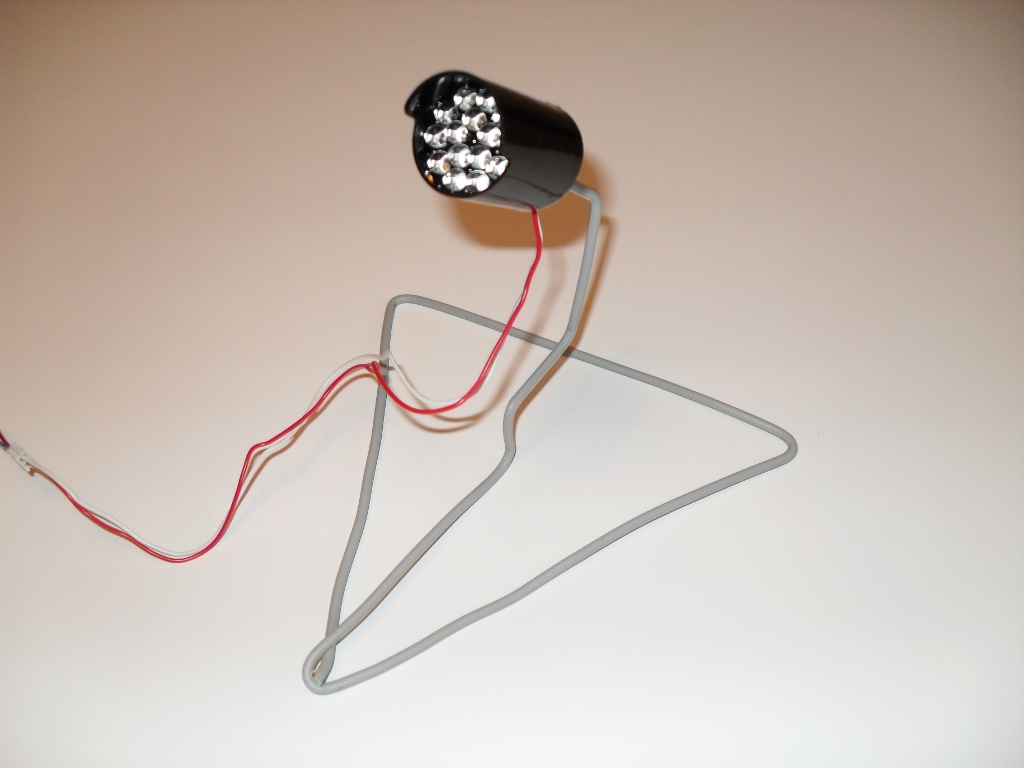
\includegraphics[width=0.4\textwidth]{../finalpres/SDC11117.JPG}}
  \subfigure[Glasses: Front view]{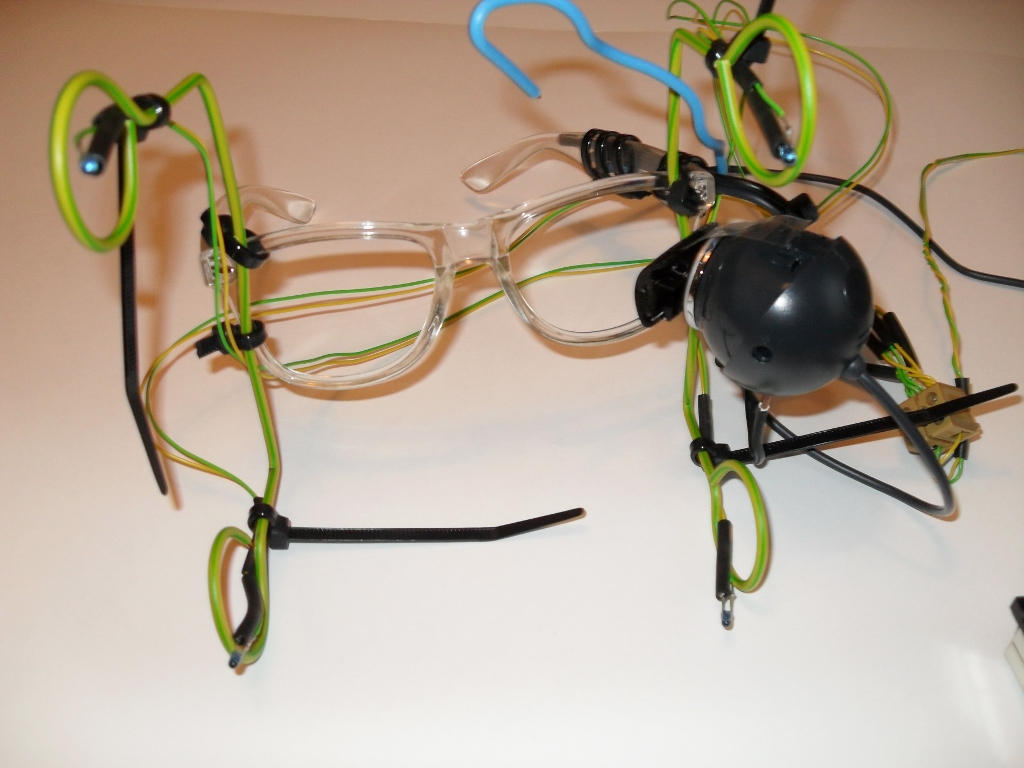
\includegraphics[width=0.4\textwidth]{../finalpres/SDC11119.JPG}}
  \subfigure[Glasses: View from above]{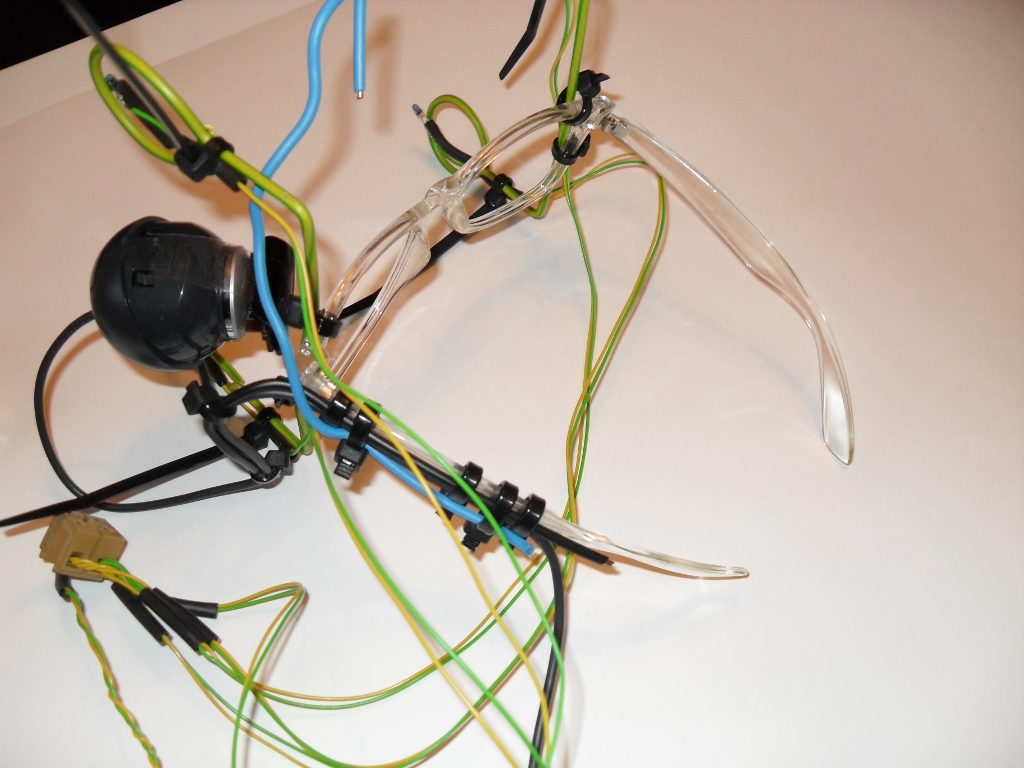
\includegraphics[width=0.4\textwidth]{../finalpres/SDC11121.JPG}}
  \subfigure[Glasses: Another view! Yey!]{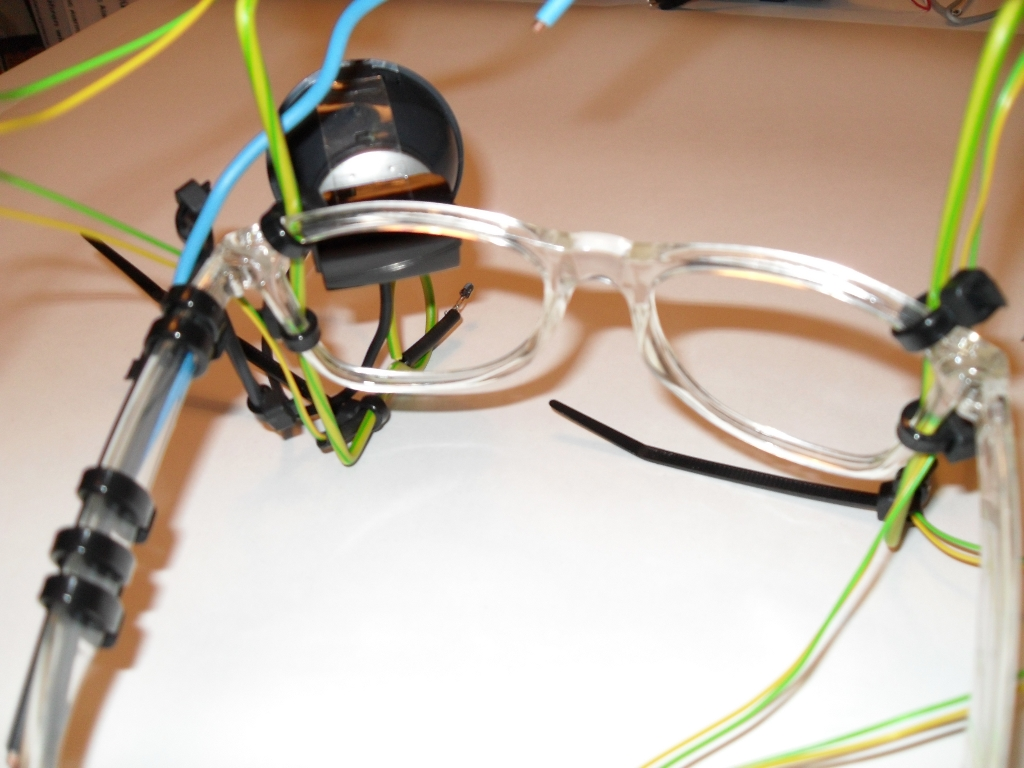
\includegraphics[width=0.4\textwidth]{../finalpres/SDC11122.JPG}}
  \caption{Hardware setup}\label{fig:hardware}
\end{figure}

\subsection{Software}

\subsubsection{Basic Principle}
\begin{figure}[H]
  \centering
  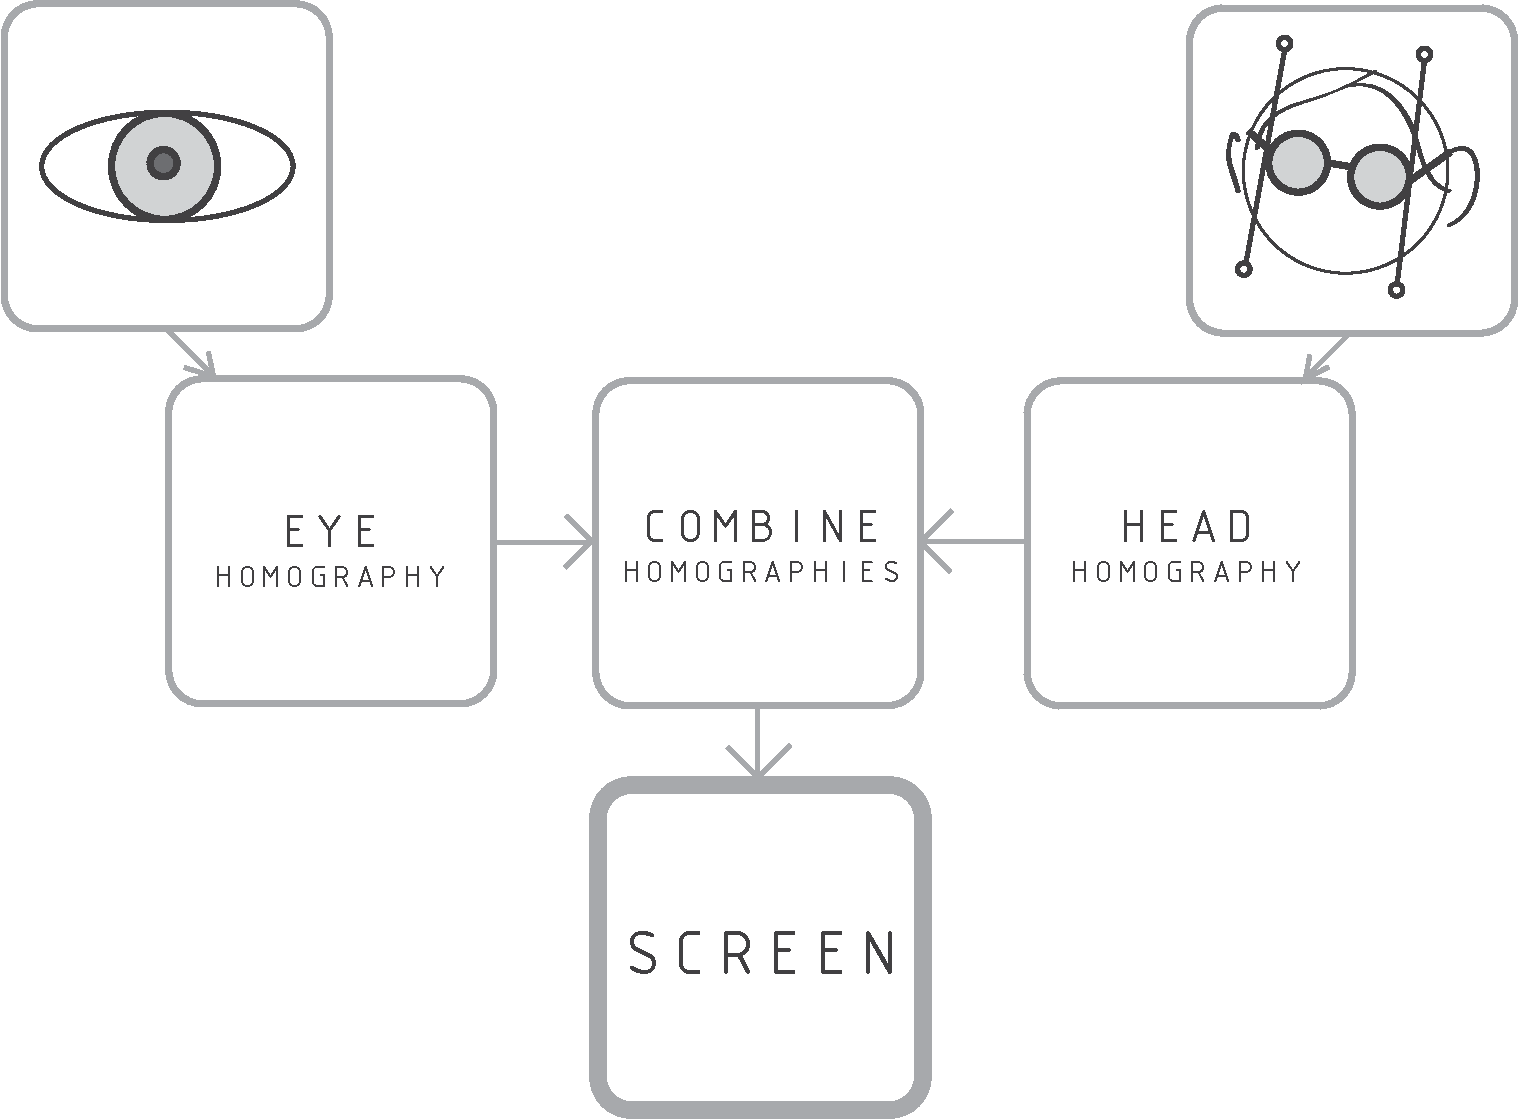
\includegraphics[width=0.9\textwidth]{../finalpres/01c.pdf}
  \caption{Basic principle of the mapping process}\label{fig:basic}
\end{figure}
The primary part necessary for proper mapping is the estimation of the homography that consists basically of two different homographies as illustrated in Fig.~\ref{fig:basic}. 
The first one is based on the image captured by the head camera which shows the four markers, while the second one is estimated using the frame showing the pupil.

The idea of using two homographies is to compensate for the error occuring due to head movement.

Computing the head homography gives us an idea of the position of the head relative to the position of the head at calibration time. 

%We need to compute the head homography and use that information to have a stable reference frame for the mapping of the pupil. 

%This is achieved with a calibration routine. 
%The user has to look at certain defined points on the screen. 
%At every point the position of the pupil is determined. 
%This information is then used to compute the homography from the pupil position to the screen using the RANSAC algorithm implemented in OpenCV. 

\subsubsection{The math}

The basic idea is to find a mapping $H$ that transforms the pupil position onto the screen, independent of the head position.

\begin{equation}
  x_\mathrm{screen} = H x_\mathrm{eye}
  \label{eq:basic}
\end{equation}

In the calibration procedure, the relationship between the pupil position and the position at the screen is estimated. Therefore the user has to look at several points on the screen. For each point, the pupil position is recorded and a homography is estimated from this information.

To include the relative head position in the calibration process, the position of the pupil $x_\mathrm{eye}$ is first mapped into a new reference frame based on the current position of the head which is given by the head's homography $H_\mathrm{calib-head}$:

\begin{equation}
  x_\mathrm{screen} = H_\mathrm{calib} (H_\mathrm{calib-head} x_\mathrm{eye})
\end{equation}

Now, $H_\mathrm{calib}$ represents the mapping of the pupil position in the new reference frame given by the head position, to the screen. One can think of $H_\mathrm{calib}$ as being composed of $H_\mathrm{eye}$ and the inverse of $H_\mathrm{calib-head}$:

\begin{equation}
  H_\mathrm{calib} = H_\mathrm{eye} H_\mathrm{calib-head} ^{-1}
\end{equation}

where $H_\mathrm{eye}$ represents the direct homography from the pupil position to the screen without considering the head position, provided the head position didn't change.

So, in case of no head movement, the mapping equation degenerates to:
% vielleicht ein besseres wort als degenerate finden

\begin{equation}
  x_\mathrm{screen} = H_\mathrm{eye} H_\mathrm{calib-head} ^{-1} H_\mathrm{calib-head} x_\mathrm{eye}
\end{equation}

\begin{equation}
  x_\mathrm{screen} = H_\mathrm{eye}  x_\mathrm{eye}
\end{equation}

In case the head moved since the calibration routine, the eye position is first mapped to the new reference frame based on the current head homography. Then, the estimated homography $H_\mathrm{calib}$ is applied.

\begin{equation}
  x_\mathrm{screen} = H_\mathrm{calib}H_\mathrm{head}x_\mathrm{eye} 
\end{equation}

Filling in the decomposed calibration homography leads to:

\begin{equation}
  x_\mathrm{screen} = H_\mathrm{calib}H_\mathrm{head}x_\mathrm{eye} = H_\mathrm{eye} H_\mathrm{calib-head} ^{-1} H_\mathrm{head} x_\mathrm{eye}
\end{equation}

We see that this takes care of the new head position. Therefore, we are able incorporate the position of the head relative to the position the head had at calibration time by implicitly calculating the relative head homography $H_\mathrm{rel-head}$.

\begin{equation}
  H_\mathrm{rel-head} = H_\mathrm{calib-head}^{-1} H_\mathrm{head}
\end{equation}

\subsubsection{Tracking of the pupil}
\begin{figure}[H]
  \centering
  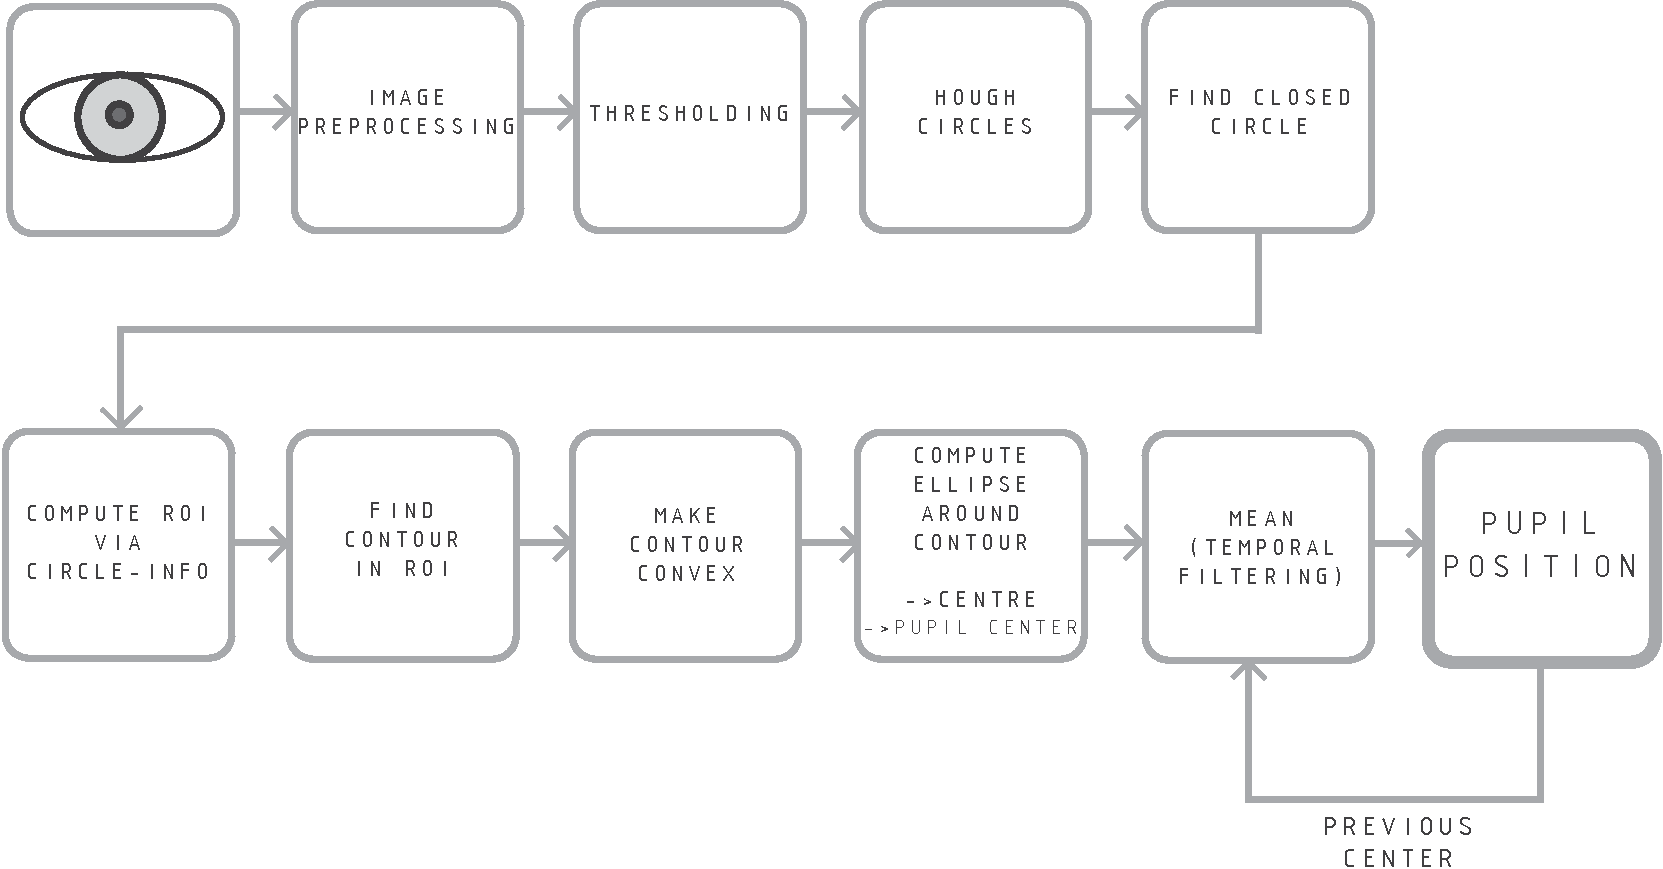
\includegraphics[width=0.9\textwidth]{../finalpres/02c.pdf}
  \caption{Pupil tracking}\label{fig:pupil}
\end{figure}
As shown in Fig.~\ref{fig:pupil} the first step is to perform several image preprocessing steps on the image aquired by the eye camera. First, the image is converted into the YCrCb color space. The frame is also cropped to a size of 120$\times$100 pixels in order to get rid of unwanted objects like the glasses.
For all the following steps only the Y-Channel is used, as this channel holds the most important information of the captured frame. 
On this channel histogram equalization is performed to increase the contrast. 
Eroding the luminance image removes small reflections of the infrared LEDs on the pupil. 
A Gaussian blurring filter takes care of noise in the current frame. 

To segment the pupil from the background, tresholding on the preprocessed image is performed. 
The segmented image is then passed to the OpenCV function \texttt{HoughCircles()}. 
Several restrictions are passed to this function as well in order to assure that no false positives occur. 
In case more than one circle is found, the closest to the previous position gets chosen as next pupil center.
The center found by the \texttt{HoughCircles()} function is not very robust and is therefore not suited to represent the center of the pupil for the tracking process.
Therefore, the information of the Hough space is only used to define a region of interest around the pupil. 
Within this ROI the contour around the pupil is computed by \texttt{findContours()}. 
The function \texttt{convexHull()} returns the convex hull around the pupil, since in some frames, reflections in the pupil cause the contour to be non-convex.
The final step is to fit an ellipse around the contour points (\texttt{fitEllipse()}).
The center of the ellipse is the center of the pupil in the current frame. 
This turns out to perform very well. 

To further smooth the tracking, temporal filtering by computing the mean of the center of the current frame with the center of the previous frame is performed as well. 
Although this slows down the tracking a bit, it is still fast enough for normal use.

\subsubsection{Tracking of the head}
\begin{figure}[H]
  \centering
  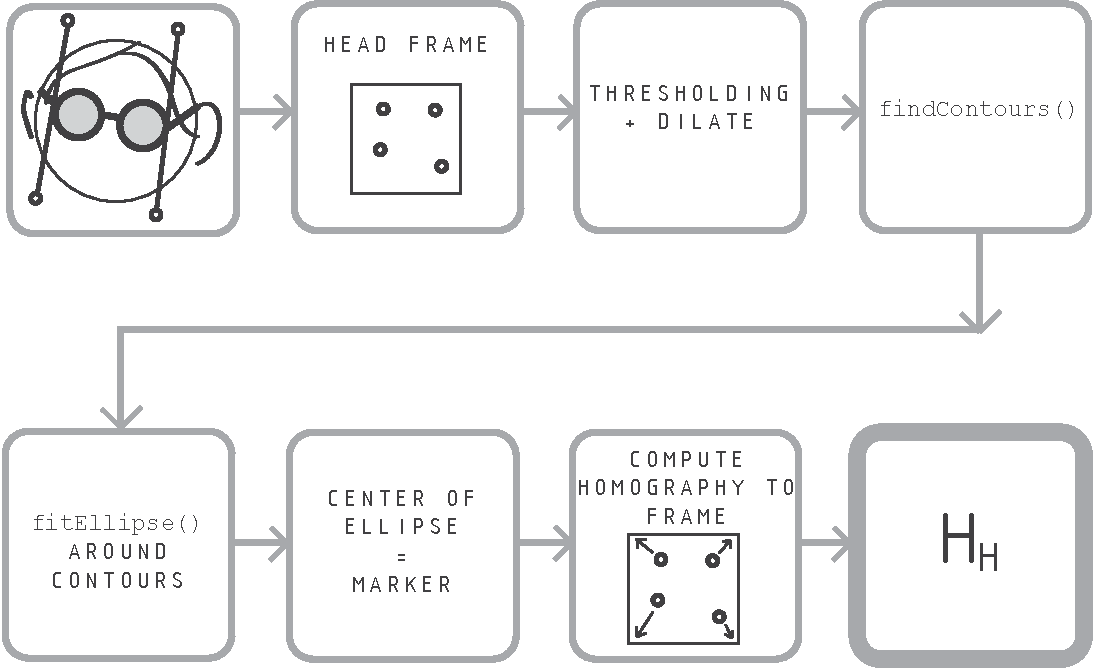
\includegraphics[width=0.9\textwidth]{../finalpres/03c.pdf}
  \caption{Head tracking}\label{fig:head}
\end{figure}

The tracking of the head (Fig.~\ref{fig:head}) is based on a filtered image (IR bandpass filter) that is captured by a built-inwebcam. The use of this filter -- in combination with the already built-in IR-filter -- leads to an suppressed infrared image of the head.
In other words: in this image only the four IR-LEDs (bright dots) can be seen and are used to calculate the homography. 
To be able to do that we perform several steps to prepare the image for the tracking and make the results as stable as possible.

To suppress side effects and noise the image is transfored to a grayscale image and thresholded. 
After that we dilate the image to increase the area of the small IR-dots. Originally the captured dots have the size of a few pixels, therefore, in order to increase the stability of the following steps, the size of the dots has to be increased. 
The shape of these dots is not optimal for the function \texttt{HoughCircles()} that was used in tracking the pupil, therefore another approach is used. 

Since the nature of the problem assures that the frame after these preprocessing steps shows just the markers, it is possible to compute the contours around the points using \texttt{findContours()}, without having to deal with any clutter. 
In case four separate contours are found (which is necessary in order to compute a homography), we can fit an ellipse around these points using \texttt{fitEllipse()}. Again, similar to the pupil tracking, the centers of the ellipses represent the centers of the points.

This information is sufficient to compute the head homography
 
%\begin{Verbatim}[numbers=left,fontsize=\small]
  %CODE
%\end{Verbatim}
